\documentclass{article}
\usepackage{tikz}
\usepackage{pgfplots}
\usepackage{xcolor}
\usepackage{svg}
\usepackage{amsmath}
\usepackage{array}
\usepackage[skins]{tcolorbox}
\usepackage[version=4]{mhchem}
\usepackage[a4paper, total={6in, 9in}]{geometry}
\usepackage{fourier}
\usepackage{xymtex}
\usepackage{textcomp}
\usepackage{eurosym}
\usepackage{caption}
\usepackage{longtable}
\usepackage{float}
\usepackage{attachfile}
\usepackage{multirow}

\captionsetup[table]{name=\textit{Tabella}}
\pagenumbering{gobble}

\title{Relazione di laboratorio - pendolo di Kater}
\author{Federico Cesari}
\date{Marzo 2024}\author{Fe\author{Federico Cesari}
	\date{Marzo 2024}derico Cesari}
\date{Marzo 2024}




\begin{document}
	\begin{titlepage}
	\begin{center}
		\vspace*{1cm}
		
		\textbf{\LARGE Relazione di laboratorio - Pendolo semplice}
		
		\vspace{0.3cm}
		\large \textit{Misura del periodo di un pendolo semplice} \\
		
		\vspace{0.5cm}
		\Large Federico Cesari \\
		
		\small 1096759 
		\vspace{0.2cm}
		
		\small Gruppo 5
		
		
		\vspace{3cm}
		\begin{center}
			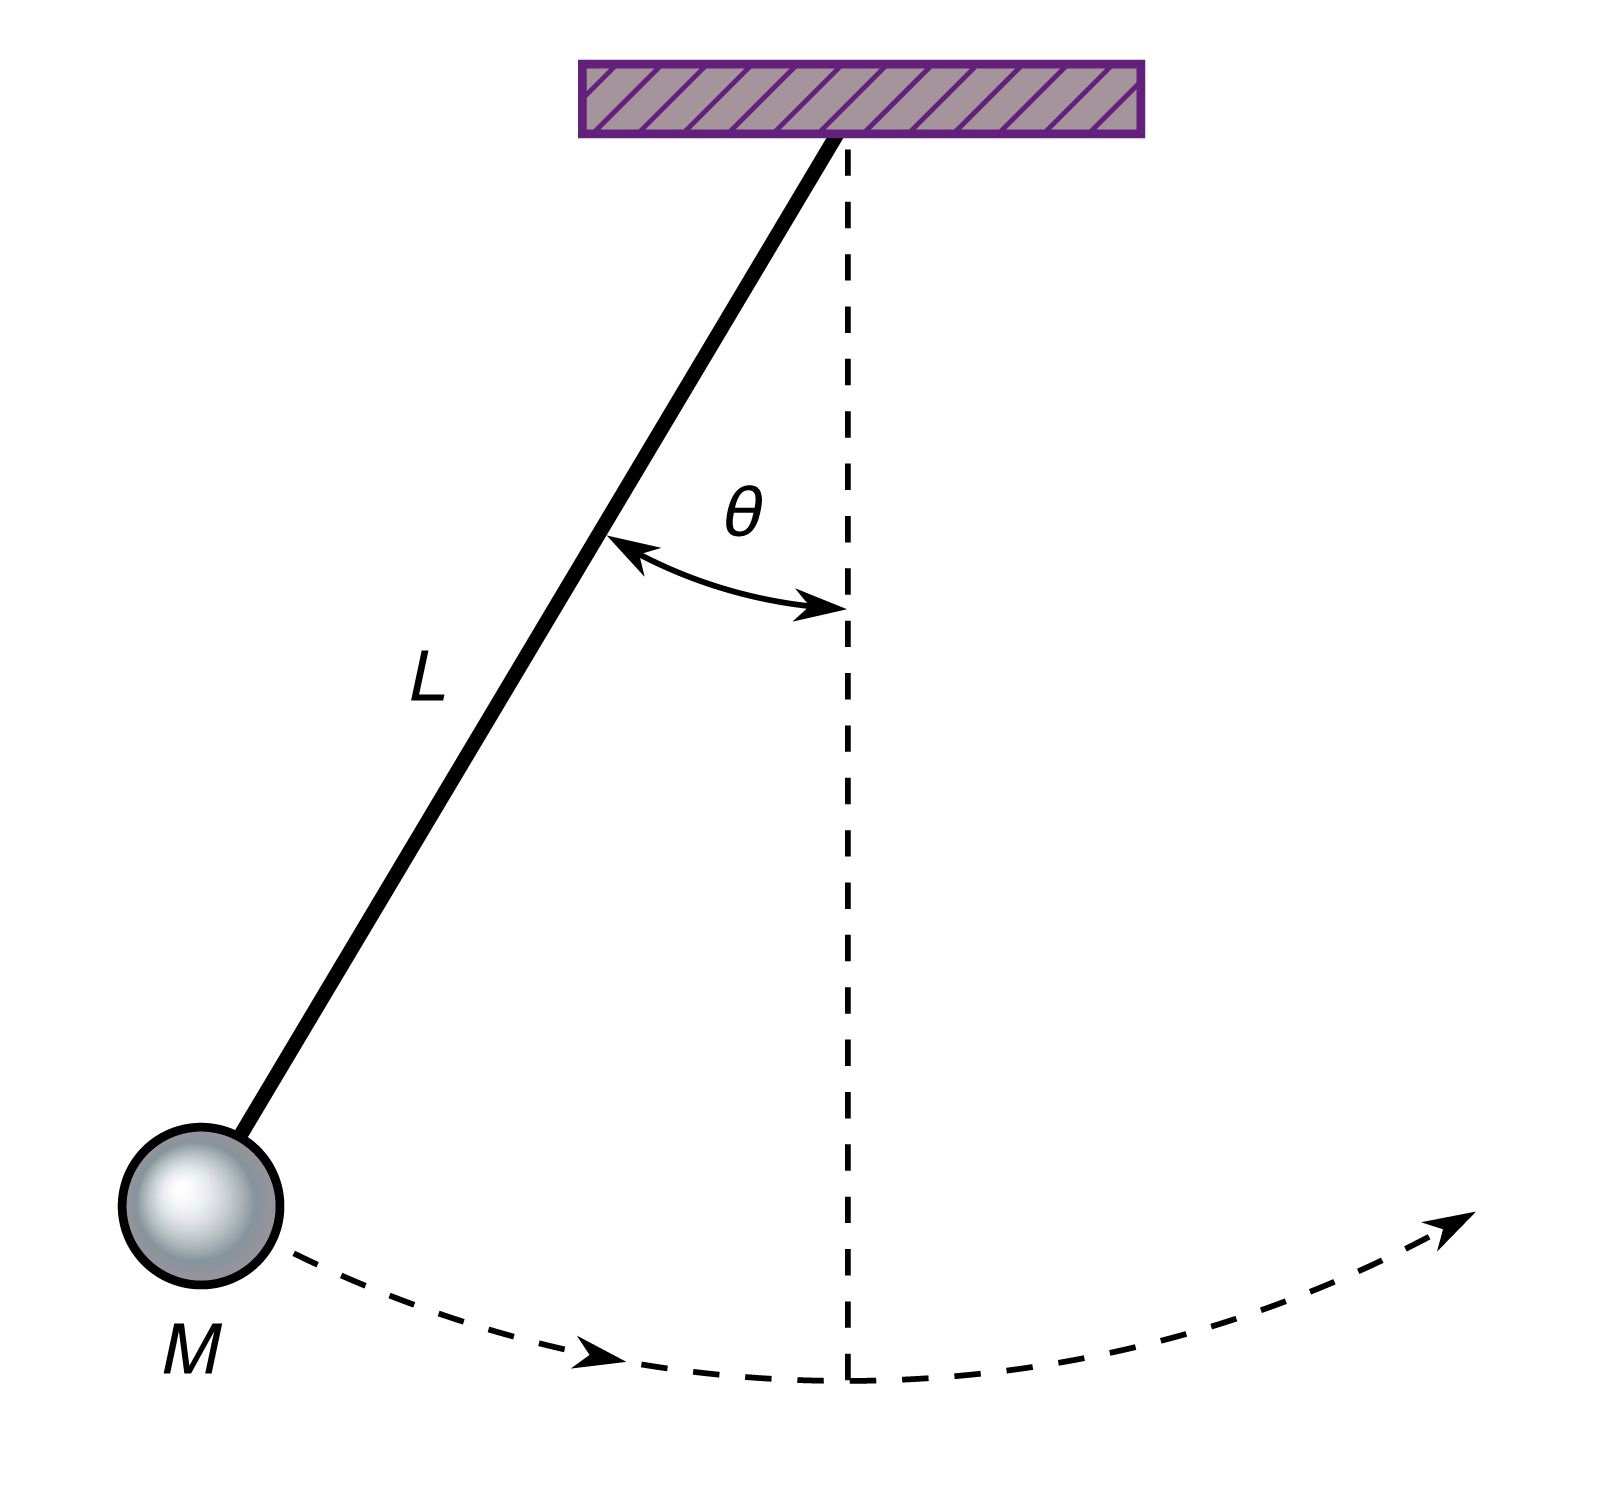
\includegraphics[scale=0.1]{IMG_0200.jpeg}	
		\end{center}
		
		
		
		\vfill
		
		
		
		corso A\\
		Università degli studi di Torino, Torino\\
		4 aprile 2024\\
		
		
	\end{center}
\end{titlepage}
	Scopo : misurare il rate 
	
	Rilevatore di radiazioni: contatore geiger
	rotaia con uranile a 3cm
	
	Calcolare il rate del fondo: rapporto tra media e deviazione standard e tempo porta.
	
	\section{Test $\chi^2$}
	!incertezza per somma e differenza è la radice quadrata della somma dei quadrati delle incertenza. \\
	
	\begin{enumerate}
		\item 	rate fondo (tempo porta = 1s): $RF(1sec) = 0.305 \pm 0.014 s^{-1}$. (\textit{nonostante preferisca una sola cifra significativa per l'errore lascio 0.014, sottostimerei di troppo se arrotondassi}.)
		\item rate fondo + sorgente (tempo porta = 1s): $RFS(<1sec) = 3.145 \pm 0.045 s^{-1}$
	\end{enumerate}
	\[
	RS(1sec) = RFS(1sec) - RF(1sec) 
	\]

	con errore
	\[
	\delta_{RS(1sec)} =\sqrt{\delta_{RFS(1sec)}^2 + \delta_{RF(1sec)}^2}
	\]
	
m

	
	
\end{document}
